\documentclass{article}

\usepackage{todonotes}

%\usepackage[disable]{todonotes}
\newcommand{\todot}[2][]{\todo[color=red!20!white,#1]{#2}}
\newcommand{\todof}[2][]{\todo[color=orange!20!white,#1]{#2}}


%%%%%%%%%%%%%%%%%%%%%%%%%%%%%%%%
% PACKAGES
%%%%%%%%%%%%%%%%%%%%%%%%%%%%%%%%
\usepackage{times}
\usepackage{fullpage}
\usepackage{latexsym}
\usepackage{amsmath}
\usepackage{amssymb}
\usepackage[boxed]{algorithm}
\usepackage{algpseudocode}
\usepackage{mathtools}
\usepackage{accents}
\usepackage{tikz}
\usepackage{pgfplots}
\usepackage{dsfont}
\usepackage[bf]{caption}
\usepackage{hyperref}
\hypersetup{
    bookmarks=true,         % show bookmarks bar?
    unicode=false,          % non-Latin characters in AcrobatÕs bookmarks
    pdftoolbar=true,        % show AcrobatÕs toolbar?
    pdfmenubar=true,        % show AcrobatÕs menu?
    pdffitwindow=false,     % window fit to page when opened
    pdfstartview={FitH},    % fits the width of the page to the window
    pdftitle={My title},    % title
    pdfauthor={Author},     % author
    pdfsubject={Subject},   % subject of the document
    pdfcreator={Creator},   % creator of the document
    pdfproducer={Producer}, % producer of the document
    pdfkeywords={keyword1} {key2} {key3}, % list of keywords
    pdfnewwindow=true,      % links in new window
    colorlinks=true,       % false: boxed links; true: colored links
    linkcolor=red,          % color of internal links (change box color with linkbordercolor)
    citecolor=blue,        % color of links to bibliography
    filecolor=magenta,      % color of file links
    urlcolor=cyan           % color of external links
}
\usepackage{comment}
\usepackage{amsthm}
\usepackage{natbib}
\usepackage[capitalize]{cleveref}
\usepackage{graphicx}
\usepackage{parskip}
\usepackage{tikz} 
\usetikzlibrary{arrows,positioning} 
\pgfarrowsdeclarecombine{ring}{ring}{}{}{o}{o}
\DeclareMathOperator{\ringarrow}{\raisebox{0.5ex}{\tikz[baseline]{\draw[ring->](0,0)--(2em,0);}}}
%%%%%%%%%%%%%%%%%%%%%%%%%%%%%%%%
% MACROS
%%%%%%%%%%%%%%%%%%%%%%%%%%%%%%%%
\newcommand{\defined}{\vcentcolon =}
\newcommand{\rdefined}{=\vcentcolon}
\newcommand{\E}{\mathbb E}
\newcommand{\Var}{\operatorname{Var}}
\newcommand{\calF}{\mathcal F}
\newcommand{\sr}[1]{\stackrel{#1}}
\newcommand{\set}[1]{\left\{#1\right\}}
\newcommand{\ind}[1]{\mathds{1}\!\!\set{#1}}
\newcommand{\argmax}{\operatornamewithlimits{arg\,max}}
\newcommand{\argmin}{\operatornamewithlimits{arg\,min}}
\newcommand{\floor}[1]{\left \lfloor {#1} \right\rfloor}
\newcommand{\ceil}[1]{\left \lceil {#1} \right\rceil}
\newcommand{\eqn}[1]{\begin{align}#1\end{align}}
\newcommand{\eq}[1]{\begin{align*}#1\end{align*}}
\newcommand{\Ber}{\operatorname{Bernoulli}}
\renewcommand{\P}[1]{\operatorname{P}\left\{#1\right\}}
\newcommand{\bigomega}[1]{\Omega\left( #1 \right)}

\renewcommand{\Pi}[1]{P_i\left( #1 \right)}
\newcommand{\Pu}[1]{P_{unif}\left( #1 \right)}
\newcommand{\Ps}[1]{P_{*}\left( #1 \right)}
\newcommand{\Ei}[1]{\E_i\left[ #1 \right]}
\newcommand{\Eu}[1]{\E_{unif}\left[ #1 \right]}
\newcommand{\Es}[1]{\E_{*}\left[ #1 \right]}
\renewcommand{\r}{\boldsymbol{r}}
\renewcommand{\log}[1]{lg\left( #1 \right)}
\newcommand{\kl}[2]{KL\left(#1 || #2 \right)}

%%%%%%%%%%%%%%%%%%%%%%%%%%%%%%%%
% THEOREMS
%%%%%%%%%%%%%%%%%%%%%%%%%%%%%%%%
\theoremstyle{plain}
\newtheorem{theorem}{Theorem}
\newtheorem{proposition}[theorem]{Proposition}
\newtheorem{lemma}[theorem]{Lemma}
\newtheorem{corollary}[theorem]{Corollary}
\theoremstyle{definition}
\newtheorem{definition}[theorem]{Definition}
\newtheorem{assumption}[theorem]{Assumption}
\newtheorem{remark}[theorem]{Remark}
\newtheorem{example}[theorem]{Example}
 \tikzset{
    %Define standard arrow tip
    >=stealth',
    %Define style for boxes
    observed/.style={
           circle,
           rounded corners,
           draw=black, thick,
           minimum width=2.2em,
           minimum height=2.2em,
           font=\footnotesize,
           text centered,
           },
     latent/.style={
           circle,
           rounded corners,
           draw=black, thick, dashed,
           minimum width=2.2em,
           minimum height=2.2em,
           font=\footnotesize,
           text centered,
           fill=black!10!white
           },
    target/.style={
           circle,
           rounded corners,
           draw=black, thick,
           minimum width=2.2em,
           minimum height=2.2em,
           font=\footnotesize,
           text centered,
           fill=black!20!white,
           },
    observedrect/.style={
           rectangle,
           rounded corners,
           draw=black, thick,
           minimum width=6em,
           minimum height=2em,
           font=\footnotesize,
           text centered,
           },
     targetrect/.style={
           rectangle,
           rounded corners,
           draw=black, thick,
           minimum width=6em,
           minimum height=2em,
           font=\footnotesize,
           text centered,
           fill=black!20!white,
           },
     empty/.style={
           circle,
           rounded corners,
           minimum width=.5em,
           minimum height=.5em,
           font=\footnotesize,
           text centered,
           },
    % Define arrow style
    pil/.style={
           o->,
           thick,
           shorten <=2pt,
           shorten >=2pt,},
    sh/.style={ shade, shading=axis, left color=red, right color=green,
    shading angle=45 }   
}


\begin{document}
\def\ci{\perp\!\!\!\perp}



\section{Lower bound on regret for K-armed bernoulli bandits}

For any horizon $T$ and number of arms $K$, there exists a strategy for choosing rewards such that the expected regret for any algorithm is $\bigomega{\sqrt{TK}}$. This strategy is oblivious to the algorithm and assigns rewards at random according to some distribution. Thus the regret bound applies to stochastic and adversarial bandits.

\begin{theorem}
There exits a distribution over rewards such that: 
\eqn {
R(T) \geq \frac{1}{20}\min{\{\sqrt{KT},T\}}
}
\end{theorem}

\begin{proof}

Consider a set of environments indexed by $i$. In environment $i$ action $i$ is the 'good' action. All other arms are slightly worse. 
\begin{itemize}
\item  In environment $i$, $r_{i,t} \sim Bernoulli(\frac{1}{2}+\epsilon)$ and $r_{j,t} \sim Bernoulli(\frac{1}{2}) \;\; \forall j \neq i$ 
\item $\Pi{.}$ is the probability with respect to environment $i$
\item $\Pu{.}$ is the probability with respect to an environment in which the expected reward for \textbf{all} arms is $\frac{1}{2}$
\item $\Ps{.}$ is the probability with respect to an environment sampled uniformly at random from $\set{1...K}$
\item $r_t$ is the reward received at time $t$
\item $\boldsymbol{r}^t = <r_1,...,r_t>$ is the history of rewards received upto time $t$
\item A is the algorithm, maps $\boldsymbol{r}^{t-1} \rightarrow i_t$
\item $N_i$ is a random variable representing the number of times action $i$ is selected by the algorithm.
\item $G_A = \sum_{t=1}^T r_t$ is the total reward for the algorithm
\item $G_{max}$ is the total reward for playing the optimal arm in every timestep. 

\end{itemize}

\begin{lemma}
\label{lem:N_not_too_big}
For any arm $i$,
\eqn{
\Ei{N_i} -\Eu{N_i} \leq  \frac{T}{2}\sqrt{-\ln({1-4\epsilon^2})\Eu{N_i}}
}

This says that the number of times we expect to play arm $i$ in the environment in which it is optimal is not too much greater than the number of times we expect to play it if all arms are equal. 

\begin{proof}
\eqn{
\Ei{N_i} -\Eu{N_i} = & \sum_{\r \in \set{0,1}^T}N_i(\r)\left(\Pi{\r} - \Pu{\r} \right) \qquad \leftarrow \text{definition of expectation}\\
\leq & \sum_{\r:\Pi{\r} \geq \Pu{\r}}N_i(\r)\left(\Pi{\r} - \Pu{\r} \right) \qquad \leftarrow \text{dropped only -ive terms}\\
\leq & T\sum_{\r:\Pi{\r} \geq \Pu{\r}}\left(\Pi{\r} - \Pu{\r} \right) \qquad \leftarrow N_i \leq T \;\; \forall \r\\
 = & \frac{T}{2}|| \Pi{\r} - \Pu{\r}||_1 \qquad \leftarrow \text{see Thomas\&Cover 11.137}\\
 \leq & \frac{T}{2}\sqrt{2\ln({2})\kl{\Pu{\r}}{\Pi{\r}}} \qquad \leftarrow \text{see Thomas\&Cover 11.138}\\
  = & \frac{T}{2}\sqrt{-ln(2)\log{1-4\epsilon^2} \Eu{N_i}} \qquad \leftarrow \text{see section \ref{sec:calculation_of_divergence}}\\
    = & \frac{T}{2}\sqrt{-\ln({1-4\epsilon^2}) \Eu{N_i}} \qquad \leftarrow \text{change of base}
}

\end{proof}
\end{lemma}

\begin{theorem}
For any algorithm $A$, if the distribution over rewards is selected unifirmly at random from environments $\set{1...K}$:

\eqn {
E_*[G_{max} - G_A] \geq \epsilon\left(T - \frac{T}{K} - \frac{T}{2}\sqrt{-\frac{T}{K}ln(1-4\epsilon^2)}  \right) 
}

\begin{proof}

\eqn{
\Ei{r_t} &= \left(\frac{1}{2}+\epsilon \right)\Pi{i_t = i} + \frac{1}{2}\left(1-\Pi{i_t = i} \right) \\
& = \frac{1}{2} + \epsilon \Pi{i_t = i}\\
\implies \Ei{G_A} &= \sum_{t=1}^T \Ei{r_t} = \frac{T}{2}+\epsilon \Ei{N_i}
}

This gives us the expected gain given action $i$ is the good action in terms of the number of times the algorithm $A$ selects action $i$. The expected gain over all the environments $i$ is:

\eqn{
\Es{G_A} &= \frac{1}{K}\sum_{i=1}^K \Ei{G_A} \\
&= \frac{T}{2} + \frac{\epsilon}{K}\sum_{i=1}^K \Ei{N_i}\\
\Es{G_{max}} &= \left(\frac{1}{2}+\epsilon \right)T
}

From lemma \ref{lem:N_not_too_big}

\eqn{
\sum_{i=1}^K\Ei{N_i} & \leq \sum_{i=1}^K \left(\Eu{N_i}+ \frac{T}{2}\sqrt{-\ln({1-4\epsilon^2})\Eu{N_i}}\right)
}

Now $\sum_{i=1}^K\Eu{N_i} = \Eu{\sum_{i=1}^K N_i} = \Eu{T} = T$ 

Note: we cannot do the same with $\sum_{i=1}^K\Ei{N_i}$ as $\Ei{.}$ is with respect to a different distribution for each $i$.

\eqn{
&\implies \sum_{i=1}^K\Ei{N_i} \leq T+ \frac{T}{2} \sqrt{-\ln(1-4\epsilon^2)KT} \qquad \leftarrow \text{via Jenson's Inequality} \\
&\implies \Es{G_A} \leq \frac{T}{2} + \epsilon\left(\frac{T}{K}+ \frac{T}{2} \sqrt{-\frac{T}{K}\ln(1-4\epsilon^2)} \right) \\ 
&\implies \Es{G_{max} - G_A} \geq \epsilon\left(T - \frac{T}{K} - \frac{T}{2}\sqrt{-\frac{T}{K}ln(1-4\epsilon^2)}  \right) 
}

\end{proof}



\end{theorem}


\end{proof}

\subsection{Calculation of KL divergence}
\label{sec:calculation_of_divergence}
\eqn{
& \kl{p(x_1,...,x_n)}{q(x_1,...,x_n)} =  \sum_{i=1}^N \kl{p(x_i|\boldsymbol{x}^{i-1})}{q(x_i|\boldsymbol{x}^{i-1})} \qquad \leftarrow \text{chain rule for KL divergence} \\
& \text{where } \kl{p(x_i|\boldsymbol{x}^{i-1})}{q(x_i|\boldsymbol{x}^{i-1})} = 
\sum_{\boldsymbol{x}^{i-1}}p(\boldsymbol{x}^{i-1})\sum_{x_i}p(x_i|\boldsymbol{x}^{i-1})\log{\frac{p(x_i|\boldsymbol{x}^{i-1})}{q(x_i|\boldsymbol{x}^{i-1})}}
}

So 
\eqn {
\kl{P_{unif}}{P_i} = \sum_{t=1}^T\left(
\underbrace{\sum_{\r^{t-1}}\Pu{\r^{t-1}}}_{\text{expectation over history}}
\underbrace{\sum_{r_t \in \set{0,1}}\Pu{r_t|\r^{t-1}}\log{\frac{\Pu{r_t|\r^{t-1}}}{\Pi{r_t|\r^{t-1}}}}}_{\text{KL divergence at time t}}
\right)
}

Now 
\eqn{
\Pu{r_t|\r^{t-1}}& = \frac{1}{2} \;\; \forall \;{r_t,\r^{t-1}} \\
\Pi{r_t|\r^{t-1}}&=
\begin{cases}
(\frac{1}{2}+\epsilon)^{r_t}(\frac{1}{2}-\epsilon)^{1-r_t} & \text{ if } A(\r^{t-1}) = i\\
\frac{1}{2} & \text{ otherwise}\\
\end{cases}
}

Let $B$ be the set of histories that lead the algorithm to select the good arm, $B =\set{ \r^{t-1}:A(\r^{t-1})=i}$. Note: $\r^{t-1}$ is sufficient to determine $i_t$ for a deterministic algorithm $A$ in the bandit setting. At the first timestep $A$ will select $i_1(A)$, it then receives reward $r_1$, selects $i_2(A,r_1)$ and so on.

\eqn {
\kl{P_{unif}}{P_i} &= \sum_{t=1}^T\left(
\sum_{B}\Pu{\r^{t-1}}
\kl{\frac{1}{2}}{\frac{1}{2}+\epsilon}
+ \sum_{B^c}\Pu{\r^{t-1}}
\kl{\frac{1}{2}}{\frac{1}{2}}
\right)\\
&= \kl{\frac{1}{2}}{\frac{1}{2}+\epsilon}\sum_{t=1}^T\left(
\sum_{B}\Pu{\r^{t-1}}
\right) \qquad \leftarrow \text{ as $kl(\frac{1}{2}||\frac{1}{2}) = 0$}\\
&=\kl{\frac{1}{2}}{\frac{1}{2}+\epsilon} \sum_{t=1}^T\left(
\Pu{i_t=i}
\right)\\
&=\kl{\frac{1}{2}}{\frac{1}{2}+\epsilon}\Eu{N_i}\\
&=-\frac{1}{2}\log{1-4\epsilon^2}\Eu{N_i}
}
\pagebreak
\subsection{Jenson's inequality}
Jenson's inequality states that for a concave function $\phi$:

\eqn{
\frac{\sum_{i=1}^K \phi(x_i)}{K} \leq \phi \left(\frac{\sum_{i=1}^K x_i}{K} \right) \\
\implies \sum_{i=1}^K \sqrt{x_i} \leq \sqrt{K\sum_{i=1}^K x_i}\\
\implies  \sum_{i=1}^K \sqrt{\Eu{N_i}} \leq \sqrt{KT} \\
\implies \sum_{i=1}^K\Ei{N_i} \leq T+ \frac{T}{2} \sqrt{-\ln(1-4\epsilon^2)KT}
}

\section{Lower bound for specific feedback graph}

Now we move to considering a Bernoulli bandit problem with the feedback graph shown in figure \ref{fig:feedbackgraph}. The environments specifying rewards over arms $\set{1...K}$ are defined identically to the standard bandit case. The expected reward for $a_0$ (in all environments) is $0$ (this is the worst case).


\begin{figure}[h]
\centering
\caption{Feedback graph}
\label{fig:feedbackgraph}
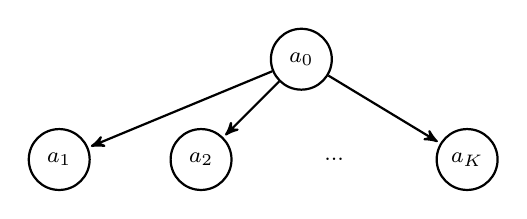
\begin{tikzpicture}[->,>=stealth',shorten >=1pt,auto,node distance=1cm,
  thick,main node/.style={observed}, hidden/.style={empty}]

 %nodes
\node[main node](1){$a_{1}$};
\node[main node, right=of 1](2){$a_{2}$};
\node[hidden, right=of 2](3){$...$};
\node[main node, right=of 3](4){$a_{K}$};
\node[main node, above right=of 2](5){$a_0$};
 \path[every node/.style={font=\sffamily\small}]
    (5) edge (1)
    	(5) edge (2)
    (5) edge (4);
	
\end{tikzpicture}
\end{figure}

As for the standard bandit case,

\eqn{
\Ei{N_i} -\Eu{N_i} \leq & \frac{T}{2}\sqrt{2\ln({2})\kl{\Pu{\boldsymbol{h}}}{\Pi{\boldsymbol{h}}}} 
}

The only difference is that the sequence of rewards $\r$ is no longer sufficient to determine $N_i$ because when we select $a_0$ we get feedback on all the other arms that does not contribute to the reward but can be leveraged by an algorithm. Therefore the KL divergence is now over distributions over the history $\boldsymbol{h}$ that includes this additional information. 

\subsection{Calculation of KL divergence}

Define 

\eqn{
h_t = 
\begin{cases}
(r_t,o_{1t},...,o_{Kt}) & \text{ if } i = 0 \\
r_t & \text{ otherwise}\\
\end{cases}
}

Where $o_{jt}$ is the observed reward for arm $j$ at timestep $t$.

\eqn {
\kl{\Pu{\boldsymbol{h}} }{\Pi{\boldsymbol{h}}} = 
\sum_{t=1}^T \kl{\Pu{h_t|\boldsymbol h^{t-1}}}{\Pi{h_t|\boldsymbol h^{t-1}}}
}

At each time step $t$, $i_t = A(\boldsymbol h^{t-1})$ There are three cases for the value of the KL divergence. 

\begin{enumerate}
\item The algorithm selects the optimal action. $i_t = i$ , (as for the standard bandit case)
\eqn{
\Pu{h_t|\boldsymbol h^{t-1}} &= \Pu{r_t|\boldsymbol h^{t-1}} = \frac{1}{2} \\
\Pi{h_t|\boldsymbol h^{t-1}} &= \Pi{r_t|\boldsymbol h^{t-1}} = 
(\frac{1}{2}+\epsilon)^{r_t}(\frac{1}{2}-\epsilon)^{1-r_t} \\
\implies kl(\frac{1}{2} || \frac{1}{2} + \epsilon)
}

\item The algorithm selects the revealing action. $i_t = 0$

\eqn {
\Pu{h_t|\boldsymbol h^{t-1}} &= B_0(r_t)\prod_{j \in \set{1...K}} B_{\frac{1}{2}}(o_j) \qquad \text{where} B_\alpha(x) \implies x \sim Bernoulli(\alpha) \\
\Pi{h_t|\boldsymbol h^{t-1}} &= B_0(r_t) \prod_{j \in \set{1...K}/i} B_{\frac{1}{2}}(o_j)B_{\frac{1}{2}+\epsilon}(o_i) \\
\implies kl(\frac{1}{2} || \frac{1}{2} + \epsilon)
}

Since the only term that differs $P_{unif}$ and $P_i$ is that for $o_i$ and,

\eqn{
\kl{\prod_{i=1}^nP_i(x_i)}{\prod_{i=1}^n Q_i(x_i)} = \sum_{i=1}^n \kl{P_i(x_i)}{Q_i(x_i)}
}


\item Otherwise. $i_t \in \set{1,..,K}/i$ , (as for the standard bandit case)
\eqn {
\Pu{h_t|\boldsymbol h^{t-1}} = \Pi{h_t|\boldsymbol h^{t-1}} = \frac{1}{2}\\
\implies kl(\frac{1}{2} ||\frac{1}{2}) = 0
}
\end{enumerate}

We divide the histories into corresponding sets. $S_1 = \set{\boldsymbol h^{t-1}:A(\boldsymbol h^{t-1})=i}$, $S_2 = \set{\boldsymbol h^{t-1}:A(\boldsymbol h^{t-1})=0}$,$S_3 = \set{\boldsymbol h^{t-1}:A(\boldsymbol h^{t-1})\in \set{1,..,K}/i}$

\eqn {
\kl{P_{unif}}{P_i} =& \sum_{t=1}^T\left(\sum_{S_1}\Pu{\boldsymbol h^{t-1}}kl(\frac{1}{2} || \frac{1}{2} + \epsilon) + 
\sum_{S_2}\Pu{\boldsymbol h^{t-1}}kl(\frac{1}{2} || \frac{1}{2} + \epsilon) +
\sum_{S_3}\Pu{\boldsymbol h^{t-1}}kl(\frac{1}{2} ||\frac{1}{2})\right) \\
=& kl(\frac{1}{2} || \frac{1}{2} + \epsilon)\sum_{t=1}^T\left(\sum_{S_1}\Pu{\boldsymbol h^{t-1}}+\sum_{S_2}\Pu{\boldsymbol h^{t-1}}  \right)\\
=& kl(\frac{1}{2} || \frac{1}{2} + \epsilon)\sum_{t=1}^T\left(\Pu{i_t = i}+\Pu{i_t=0}  \right)\\
=& kl(\frac{1}{2} || \frac{1}{2} + \epsilon)\left(\Eu{N_i}+\Eu{N_0}  \right)\\
=& -\frac{1}{2}lg(1-4\epsilon^2)\left(\Eu{N_i}+\Eu{N_0}  \right)
} 

Similarly (I think)

\eqn {
\kl{P_{i}}{P_{unif}} 
=& kl(\frac{1}{2}+\epsilon || \frac{1}{2})\left(\Ei{N_i}+\Ei{N_0}  \right)\\
=& (\frac{1}{2}lg((1+2\epsilon)(1-2\epsilon))+ \epsilon lg\left(\frac{1+2\epsilon}{1-2\epsilon}\right))\left(\Ei{N_i}+\Ei{N_0}  \right)\\
\leq & -\frac{1}{2}lg(1-4\epsilon^2)\left(\Ei{N_i}+\Ei{N_0}  \right)
} 


\subsection{Bounding regret}
We will consider only algorithms that select $N_0$ at most $\epsilon T$ times. Once an algorithm has selected $N_0$ $\epsilon T$ times, we will truncate it and play any other action at random. The regret for the non-truncated algorithm is at least $\epsilon T(\frac{1}{2}+\epsilon) \geq \frac{\epsilon T}{2}$. Truncating adds at most $(T - \epsilon T)\epsilon \leq \epsilon T$. Thus, the assumption that $N_0 \leq \epsilon T$ increases the regret by at most a constant factor of $3$. 


\eqn {
\Ei{r_t} =& (\frac{1}{2}+\epsilon)\Pi{i_t=i} + 0\Pi{i_t = 0} + \frac{1}{2}\Pi{i_t \in \set{1...K}/i}\\
=& (\frac{1}{2}+\epsilon)\Pi{i_t=i} + \frac{1}{2}(1-\Pi{i_t=i} - \Pi{i_t=0})\\
=& \frac{1}{2} + \epsilon \Pi{i_t=i} - \frac{1}{2}\Pi{i_t=0}\\
\Ei{G_A} =& \sum_{t=1}^T\Ei{r_t} = \frac{T}{2} + \epsilon \Ei{N_i} - \frac{1}{2}\Ei{N_0}\\
\Es{G_A}  =& \frac{1}{K}\sum_{i = 1}^K\Ei{G_A} = \frac{T}{2} + \frac{\epsilon}{K}\sum_{i=1}^K\Ei{N_i} - \frac{1}{2K}\sum_{i=1}^K\Ei{N_0}\\
\Es{G_{max}} =& (\frac{1}{2}+\epsilon)T}

\eqn {
\implies R(T) =& \epsilon \left(T -\frac{1}{K}\sum_{i=1}^K\Ei{N_i}\right) + \frac{1}{2K}\sum_{i=1}^K\Ei{N_0}\\
\geq & \epsilon \left(T -\frac{T}{K} - \frac{T}{2}\sqrt{-\frac{1}{K}ln(1-4\epsilon^2) (T + \sum_{i=1}^K \Eu{N_0})} \right) + \frac{1}{2K}\sum_{i=1}^K\Ei{N_0}  \\
\label{eqn:graph_regret1}
=& \epsilon \left(T -\frac{T}{K} - \frac{T}{2}\sqrt{-ln(1-4\epsilon^2) (\frac{T}{K} +  \Eu{N_0})} \right) + \frac{1}{2}\Es{N_0}\\
\geq & \epsilon \left(T -\frac{T}{K} - T\epsilon \sqrt{2(\frac{T}{K} +  \Eu{N_0})} \right) + \frac{1}{2}\Es{N_0} \qquad \text{ if } \epsilon < \frac{2}{5} \\
\geq & \frac{\epsilon}{3} \left(T -\frac{T}{K} - T\epsilon \sqrt{2T(\frac{1}{K} +  \epsilon)} \right) \qquad \text{ assuming } \Eu{N_0} \leq \epsilon T 
}

Let 

\eqn {
\epsilon = \begin{cases}
\frac{1}{4}\sqrt{\frac{K}{T}} & \text{ if } K < (16T)^{1/3}\\
(16T)^{-1/3} & \text { otherwise }
\end{cases}
}

If $K < (16T)^{1/3}$

\eqn {
R(T) \geq & \frac{1}{3}\left(\frac{1}{4}\sqrt{KT} - \frac{1}{4}\sqrt{\frac{T}{K}} - \frac{1}{16\sqrt{2}}\sqrt{4KT + K^{5/2}T^{1/2}}\right)\\
\geq & \frac{1}{3}\left(\frac{1}{4}\sqrt{KT} - \frac{1}{4}\sqrt{\frac{T}{K}} - \frac{1}{16\sqrt{2}}\sqrt{8KT}\right)\\
=& \frac{1}{3}\left(\frac{1}{8}\sqrt{KT} - \frac{1}{4}\sqrt{\frac{T}{K}}\right) \\
\geq & \frac{1}{72}\sqrt{KT} \qquad \text{ if } K > 2
}

If  $K \geq (16T)^{1/3}$
\eqn {
R(T) \geq & \frac{T^{2/3}}{3(16^{1/3})}\left(1  - \frac{1}{K} - \frac{1}{2(2^{5/6})}\sqrt{\frac{4T^{1/3}}{K}+2^{2/3}}\right)\\
 \geq & \frac{T^{2/3}}{3(16^{1/3})}\left(1  - \frac{1}{K} - \frac{1}{2(2^{5/6})}\sqrt{2(2^{2/3})}\right)\\
 = & \frac{T^{2/3}}{3(16^{1/3})}\left(1  - \frac{1}{K} - \frac{1}{2}\right)\\
 \geq & \frac{1}{46}T^{2/3} \qquad \text {if } K > 2\\
}

\pagebreak

\section{Graph changes with time}

Same as before we have a single revealing action. However, now at each timestep it reveals the rewards for a half the arms at random according to the prior probability vector $\boldsymbol{q}$


\begin{itemize}
\item Assume that $q_j \in [0,\frac{1}{2}]$ and $q_1 \leq q_2, \leq ...\leq,q_N$ 
\item Let $m \in \set{2...N} = min_i : q_j \geq \frac{1}{j}$
\item Let $M = \set{j:j \leq m}$, (the set of unbalanced arms).
\item let $D_t$ be the set of arms revealed by the revealing action at timestep $t$
\end{itemize}


\subsection{KL divergence}
As for previous section except now if the revealing action is selected, $\Pu{h_t|\boldsymbol h^{t-1}} = \Pi{h_t|\boldsymbol h^{t-1}}$ unless $i \in D_t$

The probability $P(i \in D_t)$ depends only on $\boldsymbol{q}$ (and is independent of the history at anytime step $\boldsymbol{h}$). 

So:

\eqn {
\kl{P_{unif}}{P_i} & = kl(\frac{1}{2}||\frac{1}{2}+\epsilon)\left(\Eu{N_i}+\sum_{t=1}^T\Pu{i_t=0}P(i \in D_t)\right)\\
& = kl(\frac{1}{2}||\frac{1}{2}+\epsilon)\left(\Eu{N_i}+q_i\Eu{N_0}\right)\\
\implies \Ei{N_i} & \leq \Eu{N_i} + \sqrt{2}T\epsilon \sqrt{\Eu{N_i}+q_i\Eu{N_0}} \qquad \text{assuming }  \epsilon < \frac{2}{5}
}
Let $\Es{N_i} = \sum_{i=1}^K w_i\Ei{N_i}$


\eqn {
\Es{N_i} & \leq \sum_i w_i\Eu{N_i} + \sqrt{2}T\epsilon \sqrt{\sum_i w_i\Eu{N_i}+\Eu{N_0}\sum_i w_i q_i} 
}

Choose the weights such that $P(i \in M) = \frac{1}{2}$ ie, there is a 50\% chance of choosing an environment in which the optimal arm is in the set $M$.
\eqn {
w_i = \begin{cases}
\frac{1}{2(m-1)} & \text{ if } i \leq m \\
\frac{1}{2(K-m+1)} & \text{ otherwise}
\end{cases}
}

Now $\sum_i w_i\Eu{N_i} = \Eu{\frac{1}{2(m-1)}\sum_{i=1}^{m-1}N_i+\frac{1}{2(K-m+1)}\sum_{i=m}^{K}N_i} \leq \frac{T}{2(m-1)}$, as  $m-1 < K-m+1$, since for every unbalanced arm in $m$ its partner is balanced.

\eqn {
\Es{N_i} & \leq \frac{T}{2(m-1)} + \sqrt{2}T\epsilon \sqrt{\frac{T}{2(m-1)}+\Eu{N_0}\sum_i w_i q_i}
}

\eqn{
\sum_i w_i q_i & \leq \frac{1}{2(m-1)}\sum_{i < m} \frac{1}{m} + \frac{1}{2(k-m+1)}\sum_{i \geq m} 1 = \frac{1}{2}\left(\frac{1}{m} +1\right)
}



\subsection{Bounding regret}


We can now assume that the algorithm doesn't select $N_0$ more than $\epsilon T(1-\frac{1}{2(m-1)})$ times, since we can truncate all algorithms at that point and then play arms from $i \in M$ at random.

\eqn {
R(T) &= \epsilon  \left(T -\Es{N_i}\right) + \frac{1}{2}\Es{N_0}\\
& \geq \epsilon \left (T - \frac{T}{2(m-1)} - \sqrt{2}T\epsilon \sqrt{\frac{T}{2(m-1)}+\frac{1}{2}\left(\frac{1}{m} + 1\right)\Eu{N_0}} \right)\\
& \geq \frac{\epsilon}{3} \left (T - \frac{T}{2(m-1)} - \sqrt{2}T\epsilon \sqrt{\frac{T}{2(m-1)}+\frac{1}{2}\left(\frac{1}{m} + 1\right)\epsilon T (1 - \frac{1}{2(m-1)})} \right)\\
& = \frac{\epsilon}{3} \left (T - \frac{T}{2(m-1)} - \sqrt{2}T\epsilon \sqrt{\frac{T}{2(m-1)}+\epsilon T \frac{m(2m-1)-3}{4m(m-1)}} \right)\\
& \sim \frac{\epsilon}{3} \left (T - \frac{T}{2(m-1)} - \sqrt{2}T\epsilon \sqrt{\frac{T}{2(m-1)}+\frac{\epsilon T}{2} } \right) \qquad \frac{m(2m-1)-3}{4m(m-1)} \leq \frac{9}{17} \sim \frac{1}{2}
}

No dependence on $K$ this just cannot work.


\pagebreak

\eqn {
R(T) &= \epsilon  \left(T -\frac{1}{K}\sum_{i=1}^K\Ei{N_i}\right) + \frac{1}{2K}\sum_{i=1}^K\Ei{N_0} \qquad \leftarrow \text{as before}\\
&\geq \epsilon \left(T - \frac{T}{K} - T\epsilon\sqrt{\frac{2}{K}\left(\sum_i \Eu{N_i} + \sum_{i\in M}\frac{1}{m}\Eu{N_0} + \sum_{i \notin M}\Eu{N_0} \right)}   \right)+\frac{1}{2}\Es{N_0}\\
&= \epsilon \left(T - \frac{T}{K} - T\epsilon\sqrt{2\left(\frac{T}{K} + \frac{1}{m}\Eu{N_0}\right)}   \right)+\frac{1}{2}\Es{N_0}\\
&\geq \frac{\epsilon}{3} \left(T - \frac{T}{K} - T\epsilon\sqrt{2T\left(\frac{1}{K} + \frac{\epsilon}{m}\right)}   \right) \qquad \text{assuming } \Eu{N_0} \leq \epsilon T
}


\eqn {
R(T) &= \epsilon  \left(T -\frac{1}{K}\sum_{i=1}^K\Ei{N_i}\right) + \frac{1}{2K}\sum_{i=1}^K\Ei{N_0} \qquad \leftarrow \text{as before}\\
&\leq \epsilon \left(T - \frac{T}{K} - T\epsilon\sqrt{\frac{2}{K}\left(\sum_{i\in M}\Eu{N_i} + \sum_{i \notin M}(\Eu{N_i}+\frac{1}{m}\Eu{N_0})  \right)}   \right)+\frac{1}{2}\Es{N_0}\\
&= \epsilon \left(T - \frac{T}{K} - T\epsilon\sqrt{2\left(\frac{T}{K} + \frac{1}{m}\Eu{N_0}\right)}   \right)+\frac{1}{2}\Es{N_0}\\
&\geq \frac{\epsilon}{3} \left(T - \frac{T}{K} - T\epsilon\sqrt{2T\left(\frac{1}{K} + \frac{\epsilon}{m}\right)}   \right) \qquad \text{assuming } \Eu{N_0} \leq \epsilon T
}

Let:

\eqn{
\epsilon = \begin{cases}
\frac{1}{4}\sqrt{\frac{K}{T}} & \text{if } K > m^{2/3}(16T)^{1/3} \\
m^{1/3}(16T)^{-1/3} & \text{otherwise}
\end{cases}
}
If $K < m^{2/3}(16T)^{1/3}$
\eqn {
R(T) \geq \frac{\sqrt{KT}}{12}\left(\frac{1}{2} - \frac{1}{K}\right)\\
\geq \frac{1}{72}\sqrt{KT} \qquad \text{if } K > 2
}

If  $K \geq m^{2/3}(16T)^{1/3}$
\eqn{
R(T)& \geq \frac{m^{1/3}T^{2/3}}{3(16^{1/3})}\left(\frac{1}{2} - \frac{1}{K}\right) \\
& \geq \frac{1}{46}m^{1/3}T^{2/3} \qquad \text{ if } K > 2
}

\pagebreak
\subsection{Previous Attempt at bounding regret}

If I just let $\Eu{N_0} = T$ and $\Es{N_0} = 0$, I get $R \sim \bigomega{\sqrt{T}}$ - so not tight enough. 

By similar appeal to KL divergence, we get

\eqn {
\Ei{N_0} & \geq \Eu{N_0} - \frac{T}{2}\sqrt{-ln(1-4\epsilon^2)(\Eu{N_i}+\Eu{N_0})} \\
\implies \frac{1}{K}\sum_{i=1}^K\Ei{N_0} & \geq \frac{1}{K}\sum_{i=1}^K\Eu{N_0} - \frac{T}{2K}\sum_{i=1}^K\sqrt{-ln(1-4\epsilon^2)(\Eu{N_i}+\Eu{N_0})}\\
\implies \Es{N_0} & \geq \Eu{N_0} - \frac{T}{2}\sqrt{-ln(1-4\epsilon^2)(\frac{1}{K}\sum_{i=1}^K\Eu{N_i}+\frac{1}{K}\sum_{i=1}^K\Eu{N_0})}\\
 & = \Eu{N_0} - \frac{T}{2}\sqrt{-ln(1-4\epsilon^2)(\frac{T}{K}+\Eu{N_0})}
}

\eqn{
\label{eqn:graph_regret2}
\implies R(T) \geq & 
\epsilon(T - \frac{T}{K})-(\epsilon + \frac{1}{2})\frac{T}{2}\sqrt{-ln(1-4\epsilon^2)(\frac{T}{K}+\Eu{N_0})} +\frac{1}{2}\Eu{N_0} 
}

For comparison, if we assumed $\Eu{N_0}=\Es{N_0}$ in equation \ref{eqn:graph_regret1} we would have:

\eqn{
R(T) \geq & 
\epsilon(T - \frac{T}{K})-\epsilon\frac{T}{2}\sqrt{-ln(1-4\epsilon^2)(\frac{T}{K}+\Eu{N_0})} +\frac{1}{2}\Eu{N_0} 
}

So the regret bound is pulled down by an extra  $\frac{T}{4}\sqrt{-ln(1-4\epsilon^2)(\frac{T}{K}+\Eu{N_0})}$ 


Argument that we cannot get a regret bound starting from equation \ref{eqn:graph_regret2}

Let: 
\eqn {
R_1 &= \epsilon(T - \frac{T}{K})-(\epsilon+\frac{1}{2})\frac{T}{2}\sqrt{-ln(1-4\epsilon^2)(\frac{T}{K}+\Eu{N_0})} +\frac{1}{2}\Eu{N_0} 
}

such that  $R(T) \geq R_1$ 

\eqn {
R_1 & \leq \epsilon T-(\epsilon+\frac{1}{2})\frac{T}{2}\sqrt{-ln(1-4\epsilon^2)(\frac{T}{K}+\Eu{N_0})} +\frac{1}{2}\Eu{N_0} \\
& \leq \epsilon T-\frac{1}{2}\frac{T}{2}\sqrt{-ln(1-4\epsilon^2)(\frac{T}{K}+\Eu{N_0})} +\frac{1}{2}\Eu{N_0} \\
& \leq \epsilon T-\frac{T}{4}\sqrt{4\epsilon^2(\frac{T}{K}+\Eu{N_0})} +\frac{1}{2}\Eu{N_0} \\
& \leq \epsilon T-\epsilon\frac{T}{2}\sqrt{\Eu{N_0}} +\frac{1}{2}\Eu{N_0} \\
& \leq \frac{1}{2}\left(T-\frac{T}{2}\sqrt{\Eu{N_0}}\right) +\frac{1}{2}\Eu{N_0} \\
&= \frac{1}{2}\left(2T-\frac{T^{3/2}}{2}\right) \qquad \text{if $\Eu{N_0} = T$}\\ 
& \leq 0 \qquad \text{if $T > 16$}
}



\end{document}




